\documentclass[a4paper, 12pt]{extarticle}
\usepackage[utf8]{inputenc}
\usepackage[T1]{fontenc}
\usepackage[italian]{babel}
\usepackage{amsmath}
\usepackage{amssymb,amsfonts,textcomp}
\usepackage{color}
\usepackage{array}
\usepackage{hhline}
\usepackage{hyperref}
\hypersetup{pdftex, colorlinks=true, linkcolor=blue, citecolor=blue, filecolor=blue, urlcolor=blue, pdftitle=, pdfauthor=, pdfsubject=, pdfkeywords=}
\usepackage[pdftex]{graphicx}

\pagenumbering{gobble}

\usepackage[official]{eurosym}

\setlength{\parindent}{0em}
\setlength{\parskip}{1em}

% Float figures
\usepackage{wrapfig}

% List styles
\newcommand\liststyleLSi{
\renewcommand\labelitemi{${\bullet}$}
\renewcommand\labelitemii{${\circ}$}
\renewcommand\labelitemiii{${\blacksquare}$}
\renewcommand\labelitemiv{${\bullet}$}
}

% Page layout (geometry)
\setlength\voffset{-1in}
\setlength\hoffset{-1in}
\setlength\topmargin{2.54cm}
\setlength\oddsidemargin{2.54cm}
\setlength\textheight{23.321999cm}
\setlength\textwidth{15.926cm}
\setlength\footskip{2.582cm}
\setlength\headheight{0cm}
\setlength\headsep{0cm}

% Pages styles
\makeatletter
\newcommand\ps@Standard{
  \renewcommand\@oddhead{}
  \renewcommand\@evenhead{}
  \renewcommand\@oddfoot{}
  \renewcommand\@evenfoot{\@oddfoot}
  \renewcommand\thepage{\arabic{page}}
}
\makeatother

\usepackage[usenames,dvipsnames]{xcolor}
\usepackage{framed}
\usepackage{tikz}

% nome del mese in italiano della compilazione
\usepackage{datetime}

%~ BlockQuotes serve xcolor e framed e tikz
\newcommand*\quotefont{\fontfamily{pbk}}
\usepackage{framed}
% Make commands for the quotes
\newcommand*{\openquote}{\tikz[%
remember picture,overlay,%
xshift=-15pt,yshift=-10pt]
\node (OQ) {\quotefont\fontsize{60}{60}\selectfont``};\kern0pt}
\newcommand*{\closequote}{
\tikz[remember picture,overlay,%
xshift=15pt,yshift=10pt]
\node (CQ) {\quotefont
\fontsize{60}{60}\selectfont''};}
\definecolor{shadecolor}{named}{White}
\newenvironment{shadequote}
{\begin{snugshade}
 \begin{quote}\openquote}
{\hfill\closequote\end{quote}\end{snugshade}}

% PUBLISHER LOGO -- AAHH!!! PUBLISHER!!! Use Scribus! xD
\newcommand*{\plogo}{\fbox{Gruppo Operativo Linux Empoli}}

% ~~~~~~~~~~~ FIRST PAGE BEGIN ~~~~~~~~~~~~~ %
\newcommand*{\titleAT}{\begingroup % Create the command for including the title page in the document
\newlength{\drop} % Command for generating a specific amount of whitespace
\drop=0.1\textheight % Define the command as 10% of the total text height

\rule{\textwidth}{1pt}\par % Thick horizontal line
\vspace{2pt}\vspace{-\baselineskip} % Whitespace between lines
\rule{\textwidth}{0.4pt}\par % Thin horizontal line

\vspace{\drop} % Whitespace between the top lines and title
\centering % Center all text
{
{\Huge \textbf{Uno spettro}}\\[0.5\baselineskip] % Title line 1
{\Huge \textbf{si aggira}}\\[0.5\baselineskip] % Title line 2
{\Huge \textbf{per la rete}}} % Title line 3

\vspace{0.25\drop} % Whitespace between the title and short horizontal line
\rule{0.3\textwidth}{0.4pt}\par % Short horizontal line under the title
\vspace{\drop} % Whitespace between the thin horizontal line and the author name

{\Large a cura dell'associazione
\\
\textsc{\textbf{GOLEM}}

\textit{Gruppo Operativo Linux Empoli}} % Author name

\vfill % Whitespace between the author name and publisher text
{\large
{\plogo}}\\[0.5\baselineskip] % Publisher logo

\vspace*{\drop} % Whitespace under the publisher text

\rule{\textwidth}{0.4pt}\par % Thin horizontal line
\vspace{2pt}\vspace{-\baselineskip} % Whitespace between lines
\rule{\textwidth}{1pt}\par % Thick horizontal line
\endgroup}
% ~~~~~~~~~~~ FIRST PAGE END ~~~~~~~~~~~~~ %

% ~~~~~~~~~~~ LAST PAGE FOOTER BEGIN ~~~~~~~~~~~~~~ %
\newcommand*{\footerAT}{\begingroup % Create the command for including the title page in the document

\newlength{\footdrop} % Command for generating a specific amount of whitespace
\footdrop=0.1\textheight % Define the command as 10% of the total text height

\rule{\textwidth}{1pt}\par % Thick horizontal line
\vspace{2pt}\vspace{-\baselineskip} % Whitespace between lines
\rule{\textwidth}{0.4pt}\par % Thin horizontal line

\vfill % Whitespace between the author name and publisher text
\centering{}

Un opuscolo a cura dell'associazione GOLEM\\
Rilasciato sotto licenza GPL (salvo dove diversamente specificato)\\
\texttt{golem.linux.it}

\textit{Impaginato con \LaTeX}
\\
Autoprodotto in \textit{\monthname{} \the\year}
\vspace*{\footdrop} % Whitespace under the publisher text

\rule{\textwidth}{0.4pt}\par % Thin horizontal line
\vspace{2pt}\vspace{-\baselineskip} % Whitespace between lines
\rule{\textwidth}{1pt}\par % Thick horizontal line

\endgroup}
% ~~~~~~~~~~~ LAST PAGE FOOTER END ~~~~~~~~~~~~~~ %

\begin{document}
\titleAT
\clearpage
\thispagestyle{empty}
\mbox{}
\clearpage

\section*{Il GOLEM}

\begin{wrapfigure}[11]{l}{3cm}

\includegraphics[width=3cm]{img/opuscolo-1.png}
\end{wrapfigure}

Il \textbf{GOLEM}, Gruppo Operativo Linux Empoli, è un Linux User Group
(LUG, Gruppo Utenti Linux), nato a Empoli nel Novembre 2000.

Dal 2004 è divenuto un'associazione di promozione sociale, senza scopo
di lucro, basata sull'opera volontaria e non retribuita dei suoi
membri.

L'attività di \textbf{promozione} e diffusione dell'utilizzo del
sistema \textit{GNU/Linux} e del \textit{Software Libero} si
concretizza attraverso la creazione e l'organizzazione di dibattiti,
conferenze, raccolte e scambi di documentazione, realizzazione di
pubblicazioni a carattere tecnico e divulgativo. Vengono organizzati
\textbf{corsi} per vari livelli di apprendimento, dall'alfabetizzazione
informatica all'utilizzo delle funzionalità avanzate del sistema
operativo, fino alla programmazione.

\begin{wrapfigure}{r}{6cm}
  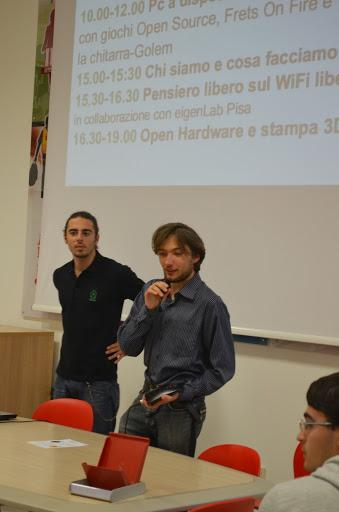
\includegraphics[width=6cm]{img/opuscolo-2.jpg}
\end{wrapfigure}

Attività distintiva del GOLEM è il \textbf{Trashware}, ovvero il
recupero di materiale informatico, definito obsoleto, per finalità
sociali, ossia la successiva donazione ad enti, altre associazioni e
privati che ne facciano richiesta. Da alcuni anni il GOLEM si è
inserito nel mondo parallelo dell'\textbf{Open Hardware}, con corsi ed
incontri relativi alla piattaforma Arduino.

Il GOLEM si riunisce nella propria \textbf{Officina Informatica} ogni
martedì, festivi esclusi, dalle 21.30 fino a notte fonda. La sede è
aperta a tutti coloro che vogliono conoscere il mondo del software
libero, oppure dare una mano nelle attività dell'associazione.

Il GOLEM è un'associazione apartitica. Lo Statuto e il Manifesto
completi sono consultabili sul nostro sito \texttt{golem.linux.it}.

\clearpage

\subsection*{Guida alla lettura}

Questo opuscolo raccoglie ordinatamente alcune considerazioni sul
software libero, supportate da alcuni articoli scritti dai volontari
del GOLEM e da altri scrittori e pensatori, che permetteranno al lettore
di comprendere l'importanza etica e pratica di queste idee.

\subsubsection*{Glossario}
\textit{Per comprendere appieno alcuni termini e meccanismi importanti}

\begin{itemize}
  \item \textbf{Software:}
    programma per computer
  \item \textbf{Hardware:}
    componenti fisici di una macchina (computer)
  \item \textbf{Licenza d'uso:}
    contratto con il quale il titolare dei diritti di sfruttamento
    economico sul programma definisce il regime giuridico di
    circolazione e le limitazioni nell'utilizzo e nella cessione
    dell'opera. La licenza è accettata implicitamente con l'utilizzo
    del software.
  \item \textbf{Licenza Libera e Software Libero:}
    tipo di licenza che si applica ad un software o ad altri tipi di
    opere intellettuali per garantirne la libertà d'utilizzo, di
    studio, di modifica e di condivisione. La prima e più famosa è la
    GNU GPL. I programmi distribuiti con licenza libera sono detti
    \textit{Software libero} (o Software Open Source) e garantiscono
    quattro libertà fondamentali:

    \begin{itemize}
      \item \textit{Libertà 0:} libertà di eseguire il programma per
        qualsiasi scopo.
      \item \textit{Libertà 1:} libertà di studiare il programma e
        modificarlo.
      \item \textit{Libertà 2:} libertà di ridistribuire copie del
        programma in modo da aiutare il prossimo.
      \item \textit{Libertà 3:} libertà di migliorare il programma e di
        distribuirne pubblicamente i miglioramenti, in modo tale che
        tutta la comunità ne tragga beneficio.
    \end{itemize}

  \item \textbf{Software proprietario:}
    Programmi la cui licenza consente al beneficiario il suo utilizzo
    sotto particolari condizioni e impedendone la modifica, la
    condivisione, lo studio e la ridistribuzione.

  \item \textbf{Codice sorgente:}
    Detto anche \textit{sorgente} o \textit{listato}, è il testo, in
    forma umanamente leggibile, della sequenza di istruzioni di un
    programma. Volendo fare un paragone culinario, è la "ricetta" che
    permette di "cucinare" il programma. Affinché il programma possa
    essere effettivamente eseguito, il codice sorgente deve essere
    tradotto in \textit{linguaggio macchina} o \textit{codice binario}.

\end{itemize}

\clearpage

\section*{Cos'è l'Open Source}
\begin{shadequote}
Il Software Libero è software che rispetta la libertà degli utenti e la
comunità. In breve, significa che \textbf{gli utenti hanno la libertà
di eseguire, copiare, distribuire, studiare, modificare e migliorare il
software}. Quindi è una questione di libertà, non di prezzo.
\par\emph{Estratto dalla definizione di Software Libero da gnu.org}
\end{shadequote}

\subsection*{Uno spettro si aggira per la rete,\newline è lo spettro del Software Libero}

Come la vecchia canzone la quale diceva che «per fare tutto ci vuole un
fiore» dobbiamo ammettere invece che «per fare tutto ci vuole il
software». Nessuno di noi può dire di non utilizzare \textbf{software}:
mentre si beve un bicchiere d'acqua si utilizza (indirettamente) il
software di produzione e di controllo di qualità della bottiglia (di
vetro o di plastica che sia), il software dei macchinari di controllo e
di analisi dell'acqua, quello del distributore che consegna a tutti i
negozi, quello della cassa del negozio dove paghiamo{\dots} Prodotti,
idee, informazioni, divertimento, sono tutti costruiti utilizzando
anche il software: anche i libri che leggete sono prodotti con carta,
inchiostro, idee e... software. Non voglio annoiare nessuno con mille
esempi, se ne possono trovare a decine.

Con questo si vuole sdoganare il falso mito che il software sia «roba
da programmatori», lontano dalla nostra vita, che lo utilizzino solo in
pochi. Ebbene no, ognuno di noi utilizza programmi informatici in dose
massiccia, che lo voglia oppure no. Proprio per questo un'innovazione
ideologica sulla produzione del software influenza e influenzerà
pesantemente la vita di noi tutti.

Non siamo abituati per niente a vederne il percorso produttivo:
un'azienda fa produrre il software ai propri programmatori e poi ne
vende la licenza d'uso. Ci si soffermi sul fatto che non vendono i
programmi: in realtà vendono il permesso di utilizzarli. Questo è il
modello di sviluppo del \textbf{Software Proprietario}.

Parallelamente al modello noto, se ne è sviluppato un secondo, per
molti anni rimasto negli atenei universitari oppure nei gruppi di
appassionati su Internet. Il modello nuovo, quello del \textbf{Software
Libero}, produce e diffonde i programmi secondo una licenza, detta GPL
- \textit{General Public License}. In effetti il motore primo della
rivoluzione è proprio questa licenza.

I programmi distribuiti sotto questa licenza possono essere
\textbf{liberamente utilizzati}, \textbf{modificati e ridistribuiti}.
Il loro codice sorgente (ovvero il testo, la ricetta che dà origine al
programma) è liberamente scaricabile da Internet, così da rendere
libera la modifica. Una volta ottenuto il programma, l'utente è libero
di farne tutto ciò che vuole, ovviamente rientrando nei termini della
licenza GPL.

Quanto detto sembra utopico e difficilmente realizzabile. Perché un
programmatore dovrebbe lavorare ore e ore per preparare dell'ottimo
software, per poi renderlo disponibile a tutti in Rete? Molti lo
pagheranno un piccolo prezzo, molti lo scaricheranno senza pagare un
euro (io lo faccio spesso!). Perché dopo una lunga fatica si rilascia
tutto il nostro lavoro, liberamente, al resto dell'umanità?

\vspace{1em}

  \begin{tabular}[h]{ccc}
  
\includegraphics[height=3.5cm]{img/opuscolo-4.png}
  &
  
\includegraphics[height=3.5cm]{img/opuscolo-5.png}
  &
  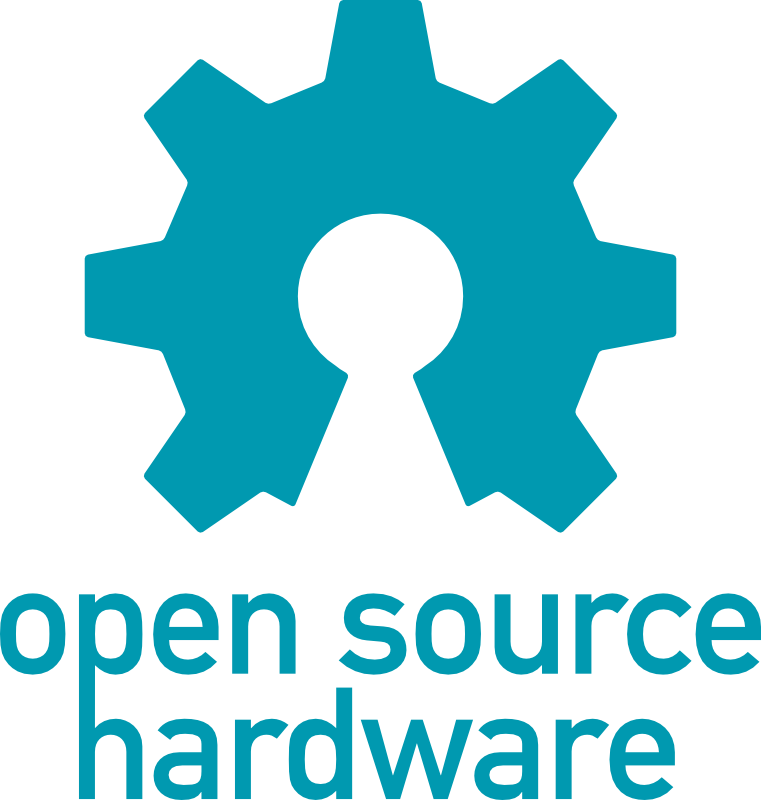
\includegraphics[height=3.5cm]{img/opuscolo-6.png}
  \end{tabular}

\vspace{1em}

Intanto, partendo dagli aspetti più nobili, c'è anche chi è impegnato
nel volontariato e dedica molta della sua vita al miglioramento delle
condizioni del prossimo: come c'è chi prepara pasti o porta barelle,
c'è chi scrive programmi. C'è poi chi passa la notte, per passione, in
una barchetta, al freddo, aspettando dei pesci improbabili, e chi passa
la notte programmando e traducendo manuali: \textit{de gustibus non
disputandum est}.

Infine si scopre che è possibile avere anche un \textbf{vantaggio}
materiale da questo lavoro: un ricercatore universitario che scrive
Software proprietario può guadagnare qualcosa, ma non può pubblicare il
suo studio. Se scrive Software Libero non incassa niente, ma può
pubblicare il suo lavoro che può essere apprezzato da altri e
permettergli di progredire nella sua carriera. Questo esempio è un po'
particolare, ma si tratteranno in seguito casi in cui un Software
Libero ha avuto o ha tuttora un grande impatto nella nostra vita.

Il Software Libero ha anche il suo rovescio della medaglia: è
scaricabile dalla Rete ma non sempre \textit{facilmente scaricabile
dalla Rete}. Bisogna imparare ad installare e configurare il nuovo
sistema, scoprire un poco del comportamento interno del proprio PC.
Questo è un piccolo prezzo da pagare. Ma da questo percorso si impara
molto sul funzionamento del proprio PC, e questo ritorna sulla buona
faccia della medaglia.

Va bene, funziona. \textit{Ma continuerà a farlo?} A volte me lo chiedo
anche io e ne sono dubbioso, ma lo stato attuale delle cose mi spinge
poi a pensare di si. I programmi di software libero, liberamente
copiabili e utilizzabili (anche senza pagare, se non si vuole farlo!)
sono cresciuti, migliorati, diffusi, fino a raggiungere i
corrispondenti software proprietari. Grandi aziende diffondono e
riutilizzano Software Libero, e le cosiddette «distribuzioni Linux»
prosperano con fortune alterne.

Qua non c'è da augurarsi che il Software Libero presto si diffonda in
tutte le case: c'è da capire \textbf{come} è possibile che lo stia già
facendo.

\begin{center}
\textit{tratto dall'articolo «Uno spettro si aggira per la rete» del GOLEM}
\end{center}

\clearpage{}

\section*{I casi di successo dell'Open Source}
I programmi rilasciati come Software Libero hanno avuto modo di
diffondersi in svariate occasioni, spesso come come alternative a
realtà proprietarie già esistenti, ma anche come novità nella sfera
dell'informatica.

I programmi qui elencati sono applicazioni mature, con una grande
comunità di supporto, guide e materiale informativo diffusi, in
italiano e molte altre lingue. In più, sono anche
\textbf{multipiattaforma}, cioè possono essere eseguiti su qualunque
sistema operativo Linux, Mac OS X o Windows, e possono essere scaricati
e installati legalmente e gratuitamente.

\begin{minipage}{.2\linewidth}
    
\includegraphics[width=0.9\linewidth]{img/opuscolo-7.png}
\end{minipage}
\begin{minipage}{.75\linewidth}
\textbf{LibreOffice} è una suite da ufficio, cioè un insieme di
programmi per la produttività personale e da ufficio: scrittura di
testi, analisi di dati e presentazioni multimediali. I suoi punti di
forza sono il vasto supporto a numerosi formati di file e la sua sempre
più capillare diffusione all'interno di uffici privati, pubbliche
amministrazioni, scuole ed enti di ricerca.\\
Sito web: \texttt{https://it.libreoffice.org}
\end{minipage}

\begin{minipage}{.2\linewidth}
    
\includegraphics[width=.9\linewidth]{img/opuscolo-8.png}
\end{minipage}
\begin{minipage}{.75\linewidth}
\textbf{Firefox} è un web browser, cioè un programma per navigare sul
Web, prodotto da Mozilla. I suoi punti di forza sono la velocità con
cui mostra le pagine e l'alto grado di personalizzazione che si può
ottenere con i numerosi componenti aggiuntivi installabili. È
disponibile anche per smartphone Android e Apple, e permette di
sincronizzare preferiti e cronologia tra i vari dispositivi.\\
Sito web: \texttt{https://www.mozilla.org/it/firefox/products/}
\end{minipage}

\begin{minipage}{.2\linewidth}
    
\includegraphics[width=.9\linewidth]{img/opuscolo-9.png}
\end{minipage}
\begin{minipage}{.75\linewidth}
\textbf{Thunderbird} è un client di posta, cioè un programma che consente di gestire, in maniera aggregata, le proprie
caselle email e i rispettivi messaggi. Il suo punto di forza è l'alto grado di personalizzazione che si può ottenere
con i numerosi compontenti aggiuntivi disponibili. Integra anche un calendario che può essere sincronizzato tra vari
dispositivi.\\
Sito web: \texttt{https://www.mozilla.org/it/thunderbird/}
\end{minipage}

\begin{minipage}{.2\linewidth}
    
\includegraphics[width=.9\linewidth]{img/opuscolo-10.png}
\end{minipage}
\begin{minipage}{.75\linewidth}
\textbf{GIMP} è un programma di fotoritocco per la modifica delle
fotografie. È arricchito con numerosi plug-in che consentono di
compiere le operazioni più disparate: dalla semplice importazione di
foto RAW all'assemblaggio di panorami. Inoltre, grazie agli script, è
possibile ripetere i ritocchi su più fotografie in maniera automatica o
interattiva.\\
Sito web: \texttt{http://www.gimp.org/}
\end{minipage}

\begin{minipage}{.2\linewidth}
    
\includegraphics[width=.9\linewidth]{img/opuscolo-11.png}
\end{minipage}
\begin{minipage}{.75\linewidth}
\textbf{Inkscape} è un programma di grafica vettoriale, cioè che
consente di realizzare loghi e disegni scalabili.\\
Sito web: \texttt{https://inkscape.org/it/}
\end{minipage}

\begin{minipage}{.2\linewidth}
    
\includegraphics[width=.9\linewidth]{img/opuscolo-12.png}
\end{minipage}
\begin{minipage}{.75\linewidth}
\textbf{VLC} è un programma per la riproduzione di musica e video. I
suoi punti di forza sono il supporto della maggior parte dei formati esistenti, la
possibilità di convertire audio e video in altri formati e la
trasmissione via rete di flussi video.\\
Sito web: \texttt{http://www.videolan.org/vlc}
\end{minipage}

\begin{minipage}{.2\linewidth}
    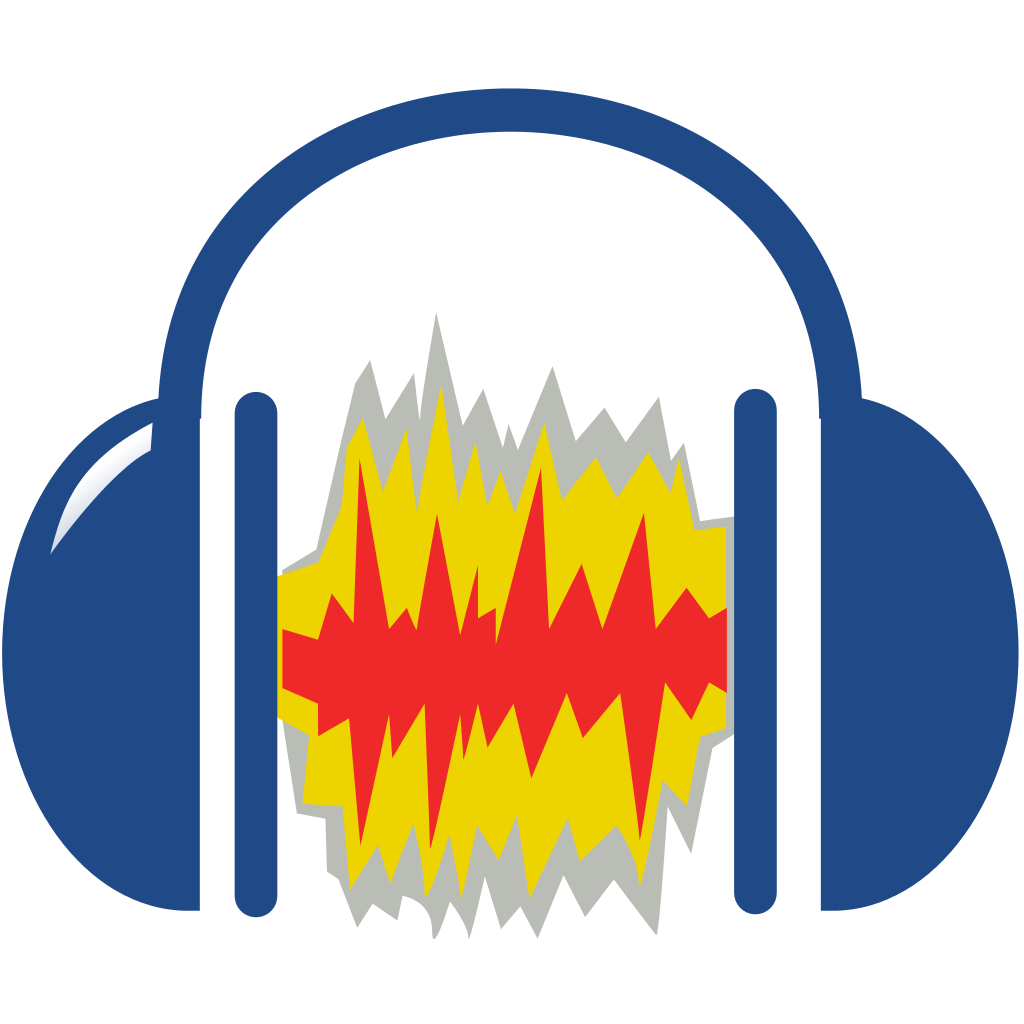
\includegraphics[width=.9\linewidth]{img/opuscolo-13.png}
\end{minipage}
\begin{minipage}{.75\linewidth}
\textbf{Audacity} è un programma di registrazione multitraccia, adatto per la registrazione di più strumenti musicali e
la modifica di canzoni. Include anche strumenti per la generazione di suoni e rumori,
per la rimozione del rumore di fondo ed il trattamento delle tracce audio.
Riesce ad importare ed esportare buona parte dei formati audio.\\
Sito web: \texttt{http://www.audacityteam.org/}
\end{minipage}

\begin{minipage}{.2\linewidth}
    
\includegraphics[width=.9\linewidth]{img/opuscolo-14.png}
\end{minipage}
\begin{minipage}{.75\linewidth}
\textbf{Arduino} è un ambiente di sviluppo per la programmazione di
schede elettroniche. Ha dato il via all'Open Source Hardware ed al
movimento Maker, consentendo a chiunque di sperimentare con
l'elettronica.\\
Sito web: \texttt{http://www.arduino.cc/}
\end{minipage}

\clearpage

\section*{Il paradigma dello sviluppo Open}

\begin{shadequote}
Ecco, questo è il mondo dei programmi liberi: un
mondo vitale, in fermento e sprecone, come solo la natura riesce ad
esserlo. Ogni rana depone una quantità innumerevole di uova per creare
solo pochi suoi simili. Ma non solo. Il Software Libero, come la
natura, si evolve. Elementi di codice (genetico o digitato),
imponderato e imponderabile, possono genialmente inserirsi in ogni
progetto, per opera di ogni libero programmatore. Infatti l'evoluzione
non ha tempi preordinati, è veloce o lenta in base alle condizioni
ambientali, a quanto è necessario o richiesto dal programma.
\par\emph{dall'articolo «Darwin contro il dottor Moreau» dell'associazione GOLEM}
\end{shadequote}

A differenza del software proprietario, il software libero appare meno
visibile, ad un'analisi superficiale.\\
Il software proprietario porta
con sé i nomi di grandi aziende multinazionali, grandi numeri che
certificano la sua diffusione, ed è ampiamente e largamente
pubblicizzato per via dell'immediato ritorno economico.\\
Il software
libero ha invece una diffusione meno centralizzata, più capillare e
sicuramente meno pubblicizzata: dà lavoro a numerose piccole imprese
locali, ma è anche al celato servizio dei grandi colossi
dell'informatica.

Il suo modello di sviluppo è \textit{caotico}, \textit{sprecone},
\textit{ridondante}: esistono molti progetti open con uno stesso
obiettivo, e programmi sviluppati per far qualcosa di "inutile". Poi,
qualche programma spicca per \textbf{originalità} e \textbf{utilità},
pian piano cresce e viene migliorato da un numero sempre più grande di
programmatori, finché diventa famoso, diffuso, e volendo anche un
business per alcune imprese. Queste imprese hanno interesse a
modificare il programma per migliorarlo, perché è grazie a quel
programma che traggono un vantaggio economico. E, nel rispetto
dell'utilizzatore finale, rilasciano le loro modifiche e contribuiscono
a migliorare il prodotto finale.

\textbf{Canonical}, \textbf{RedHat} e \textbf{SuSe} sono un esempio di
\textit{produttori} di sistemi operativi liberi, rispettivamente
\textit{Ubuntu}, \textit{RedHat Enterprise Linux} e \textit{Suse}. La
prima è riuscita ad indirizzare la sua distribuzione al grande
pubblico, soprattutto agli utenti inesperti. Le altre due invece si
rivolgono maggiormente alle aziende, e riescono ad avere dei ricavi
offrendo corsi e supporto tecnico.

Sicuramente alla base del fenomeno Web 2.0 è il progetto
\textbf{Apache}: si tratta di un server web, ovvero del motore alla
base della quasi totalità dei siti web, che lavora in coppia con
altri strumenti e linguaggi di programmazione liberi (\textit{PHP, HTML,
MySQL}). Analoghi programmi liberi vengono utilizzati da
\textit{Google}, \textit{Facebook}, \textit{Wikipedia} e persino da \textit{Microsoft}.

Ricollegandosi alle piattaforme Web, è famoso il caso di
\textbf{Wordpress}, una piattaforma open source per la creazione di
blog: la scelta di rilasciare il programma liberamente sotto la licenza
GPL viene ripagata dall'attività di hosting che la società stessa offre
e alla quale molti blogger si appoggiano. Naturalmente senza limitare
la possibilità di installare tale applicativo dove si preferisce.

Abbiamo citato Google, colosso dell'informatica che ha fatto dell'Open
Source un mestiere.
Google non produce telefoni cellulari, ma produce il
sistema operativo che gira sulla maggior parte di essi:
\textbf{Android}. Esso deve il suo successo al suo modello di sviluppo
aperto, poiché può essere modellato ed installato su una grande varietà
di smartphone e non solo: possiamo trovarlo anche su autoradio,
televisioni e decoder. Questo non accade per Apple iOS e Windows Phone:
data la loro natura chiusa sono legati a pochi dispositivi, e comunque
tutti dello stesso produttore.

Anche il browser \textbf{Google Chrome} deriva da un progetto open,
\textit{Chromium}. In questo caso, lo sviluppo dei due applicativi
procede parallelamente, e l'utente è libero di scegliere se installare
la versione col marchio Google, oppure quella \textit{più open}.

Persino \textbf{2048}, un gioco di logica per smartphone, open source, è
divenuto famoso grazie alla sua semplicità iniziale e ai numerosi fork
(versioni modificate che aggiungono funzionalità).
Il suo autore, disoccupato ai tempi in cui ha programmato l'applicazione,
si è guadagnato bene l'assunzione!

Concludiamo con il già citato progetto \textbf{Arduino}: la piattaforma
per lo sviluppo rapido di applicazioni elettroniche.
Il suo obiettivo è dare uno strumento per realizzare progetti interattivi
a chi non è esperto di programmazione ed elettronica.
In un mondo in cui queste due tecniche fanno da padrone
è stato accolto a braccia aperte.\\
Senza l'Open Source tale progetto non avrebbe avuto lo stesso successo:
è proprio grazie alla condivisione degli schemi elettrici, dei codici e
delle idee se in molti lo utilizzano.
Ma anche Arduino ha ripreso molto da \textit{Processing} e
\textit{Wiring}, due progetti (uno americano e l'altro spagnolo)
già esistenti, ed entrambi Open Source.

\clearpage

\section*{Libertà, licenze, diritti e doveri}

\textbf{Pirateria: la legalità aiuta l'Open Source, l'illegalità lo danneggia}

Il fattore che reputo essere il più importante di tutti per il successo
dei programmi Open Source è la lotta alla pirateria: infatti gli utenti
decidono di orientarsi verso l'open source quando il confronto con il
software proprietario viene fatto rispettando tutte le regole del
gioco. Scegliere fra pagare oltre 200\euro{} per avere Windows Professional
e non pagare nulla per Linux è ben diverso dallo scegliere fra Windows
piratato e Linux: io la seconda opzione la definirei
\textbf{concorrenza sleale}.

Le aziende infatti, più propense alla legalità (leggasi
\textit{costrette}), si stanno accorgendo che Libre Office è una ottima
alternativa alla suite di casa Microsoft, e di esempi simili se ne
possono fare tanti. La pirateria ha giocato un ruolo fondamentale nella
diffusione di alcuni software proprietari. Oggi invece,
paradossalmente, la diffidenza degli utenti nei confronti di Windows
sta proprio nella paura di non poter più usare il software piratato.

Non vi dice nulla la frase:
«Caspita, ho comprato il computer nuovo, ma sopra non c'è Office, me lo
installi tu?»

Io me la sono sentita dire decine di volte e ogni volta che la sento mi
fa imbestialire: molti utenti non hanno proprio la percezione del
problema, per loro Office è \textit{parte integrante} di Windows,
quindi è un prodotto gratuito, cosa che ovviamente non è affatto vera.

Installare Office non originale è un \textbf{reato}, installare Windows
non originale è un \textbf{reato}, installare Adobe Photoshop non
originale è un \textbf{reato}, ma pochi sono davvero consapevoli di
questo. Il sostegno più importante che si può dare all'open source è
proprio quello del sensibilizzare le persone sulle differenze fra il
software proprietario e piratato ed il software libero, che invece è
quasi sempre gratuito per l'utente, ma legalmente. Date a Microsoft
quel che è di Microsoft ed agli utenti una buona distribuzione Linux
ben corredata, perché solo giocando ad armi pari si potrà stabilire un
vero vincitore.

\begin{center}
\textit{articolo pubblicato su Doxaliber, rielaborato da GOLEM}
\end{center}

\clearpage

\section*{I casi di insuccesso del software proprietario}

\textbf{Dieselgate, una questione di software chiuso}

Non si parla d'altro in questi giorni: \textbf{VolksWagen} ha ammesso
di aver truccato la centralina dei propri \textbf{motori diesel} per
far finta di rispettare le severe norme anti-inquinamento negli USA e
superare in maniera fraudolenta i test di omologazione.

\subsection*{Software nel motore?}

Un \textbf{motore endotermico} è una macchina tutto sommato semplice.
Entra una miscela aria-carburante, viene compressa, avviene
un'espansione che trasforma l'energia chimica in movimento e i gas
combusti vengono espulsi. Le innovazioni nel motore a ciclo diesel sono
state tutto sommato contenute da un secolo a oggi.

Tuttavia il motore diesel è estremamente inquinante, perciò, in questi
ultimi anni si è preteso che le \textbf{emissioni} di anidride
carbonica e particolato venissero ridotte drasticamente, e questo è
stato fatto fondamentalmente con tre elementi: la \textit{marmitta
catalitica}, il \textit{filtro antiparticolato} e l'\textit{iniezione
elettronica}. Il sistema, in sé estremamente semplice, è diventato
estremamente complicato, perché i tre controlli devono per forza
lavorare assieme.

Tenere assieme il puzzle, affinché tutto funzioni bene, è piuttosto
difficile. Occorre raffinare le mappature del motore affinché, in tutte
le condizioni, esso funzioni come sperato, senza sacrificare troppo i
consumi e le prestazioni. Per forza di cose non si punta però a
creare il motore "più perfetto possibile", ma quello che
\textit{risponde meglio} ai test. Se i test sono fatti bene,
rispecchiando un modello sufficientemente realistico di un uso medio,
le due cose tendono ad avvicinarsi.

La complessità e la necessità di adattarsi alle varie condizioni fa sì
che occorra usare componenti software, cioè programmi, per adattare il
comportamento del motore ai modelli teorici. La stessa cosa avviene
anche con i dispositivi di frenata assistita, anti-bloccaggio (ABS),
per il controllo di stabilità (ESP). Insomma, il software, in buona
parte guida la nostra auto.

\subsection*{Software segreto, non ispezionabile. Qui inizia il problema.}

Il software che viene montato a bordo delle auto è dunque molto
\textbf{intelligente}, forse anche troppo. Come detto, si cerca più di
adattarsi ai test, che avvicinarsi a realizzare il motore ideale.
Come fanno molti studenti, è forte la tentazione di passare dallo
studiare per conoscere la materia, a studiare solo in funzione dei
test, e poi a studiare direttamente i test invece della materia.

Siccome i parametri in ingresso alla centralina sono molti, è stato
relativamente facile \textbf{programmare} il software per permettergli
di capire se era in presenza di un test in laboratorio. Da quanto si
sa, il software è stato addestrato a modificare i parametri di utilizzo
per rispettare i vincoli normativi anti inquinamento in presenza del
test.

A questo punto uno si domanda: ma come speravano di farla franca, non
c'è nessuno che sa leggere il software e capire che le istruzioni sono
fatte per barare? Ovviamente sì. Peccato che sia, in larga parte,
vietato.

Il software è \textbf{protetto} non solo dal copyright, ma anche da
alcune disposizioni che ne tutelano il segreto. Infatti, il codice
binario, quello che fa funzionare la centralina, non può essere
decompilato (cioè ri-tradotto in forma umanamente comprensibile) se non
in presenza di alcune particolari condizioni. Inoltre, è proibito
rimuovere le protezioni apposte dal titolare dei diritti, per cui,
anche ipotizzando di avere il diritto di modificare il software per
correggere gli errori, in presenza di un dispositivo di protezione, non
si può comunque far niente. Questa attività non è vietata a organi
ispettivi per finalità di accertamento di frodi; peccato che non sia
nei loro compiti effettuarla.

Ad ogni modo, non vi sono norme che impongano ai produttori di auto di
rendere disponibile il codice sorgente delle loro centraline alle
autorità. Senza codice sorgente, rimane solo la decompilazione, che,
oltre che attualmente illegale, è procedimento molto inefficiente e
difficile, soprattutto nei sistemi dedicati, come le centraline delle
automobili.

Esistono numerosi soggetti che avrebbero le capacità e l'interesse a
effettuare questi controlli in modo indipendente, come enti autonomi di
ricerca, associazioni di consumatori e privati cittadini, ma non lo
possono fare, perché, se lo facessero, rischierebbero azioni penali.

Mancando la seria possibilità di essere sottoposti a sanzioni e
mancando la pressione dei "controinteressati", il gioco è sbilanciato
verso l'elusione delle regole.

\subsection*{La soluzione è Open Source}

Nel caso di VolksWagen, l'inghippo non proviene da una soffiata, non
proviene da un controllo più zelante del solito, proviene proprio da un
ente autonomo incaricato di vagliare alcuni sospetti iniziali.

I tecnici dell'ente non hanno potuto osservare il codice e testarlo,
perché proibito: hanno invece creato un marchingegno che ripropone ciò
che i test dovrebbero simulare, ma con un veicolo in marcia effettiva.
Hanno fatto sull'auto quello che si chiama "studio osservazionale".

L'ente di ricerca ha scoperto che nel mondo reale i risultati erano
talmente difformi da far sospettare che non fosse un caso, ma un
risultato voluto. Hanno perciò scoperto \textit{dal di fuori} quale
fosse il vero funzionamento del software.

L'accertamento compiuto è macchinoso, e ovviamente adatto a misurare
difformità grossolane tra il comportamento atteso e il comportamento
osservato. Non è una soluzione per difformità più microscopiche, ma non
meno importanti, come per esempio una \textbf{vulnerabilità} che
consenta - come è stato recentemente dimostrato - di intervenire
direttamente dall'esterno sui parametri del motore, dei freni, dello
sterzo e, con alcuni modelli di auto, uccidere potenzialmente qualcuno
(addirittura con apparecchi radio!).

Queste vulnerabilità possono essere scoperte, con molta perizia, solo
osservando come il software è stato realizzato, e ciò sarebbe possibile
solo con la disponibilità del codice sorgente.

Il passo logico conclusivo è che il software a cui ci affidiamo per la
\textbf{salute} e la \textbf{sicurezza} dovrebbe essere \textbf{open
source}.

A tutti dovrebbe essere dato il permesso di studiarlo e verificare che
fa quello che dice, installandolo al posto di quello ufficiale. E ciò
dovrebbe valere per tutto, non solo per le auto: dai dispositivi di
voto, agli apparati elettromedicali, a tutto ciò che va sotto il nome
di "Domotica" e "Internet of Things".

L'obiezione contraria è fallace e drammaticamente smentita dai fatti:
si dice che, se si consentisse ciò, tutto sarebbe insicuro, la gente si
metterebbe a modificare il software della macchina per farla andare più
veloce e consumare di più, come se ciò non fosse già possibile in altro
modo!

Infine, il fatto di ritenere che la sicurezza si abbia
solo con il segreto, è un principio totalmente smentito da ogni teoria
scientifica sulla sicurezza. Anzi, è vero il contrario: la sicurezza si
ha solo se le insicurezze possono essere testate da molti, e non solo
dai malintenzionati.

\begin{center}
\textit{articolo scritto da Carlo Piana il 25 settembre 2015 e adattato da GOLEM\\
Rilasciato sotto licenza Creative Commons Attribuzione - Condividi allo stesso modo 4.0}
\end{center}

\clearpage
\thispagestyle{empty}
\mbox{}
\clearpage

\footerAT

\end{document}
